\documentclass[10pt,twocolumn,a4paper]{article}

\usepackage{amsfonts}
\usepackage{amsmath}
\usepackage{geometry}
\usepackage{xcolor,graphicx}
\usepackage[subfolder,cleanup]{gnuplottex}
%\usepackage{amsthm}
%\usepackage{enumitem}
%\usepackage{wrapfig}
\usepackage{subcaption}
%\usepackage{hyperref}
\usepackage{tikz}
\RequirePackage{cite}

\usetikzlibrary{patterns,decorations.pathreplacing}
\usetikzlibrary{arrows.meta}
\usetikzlibrary{shapes.arrows, fadings}

\let\originalleft\left
\let\originalright\right
\renewcommand{\left}{\mathopen{}\mathclose\bgroup\originalleft}
\renewcommand{\right}{\aftergroup\egroup\originalright}

\providecommand{\df}{\textrm{d}}
\newcommand{\diff}[3][]{\frac{\textrm{d}^{#1}#2}{\textrm{d}{#3}^{#1}}}
\newcommand{\pdiff}[3][]{\frac{\partial^{#1}#2}{\partial{#3}^{#1}}}
\newcommand{\Es}{E_{\textrm{sat}}}
\newcommand{\FT}[1]{\mathcal{F}\left\{ #1 \right\}}
\newcommand{\FTi}[1]{\mathcal{F}^{-1}\left\{ #1 \right\}}
\newcommand{\Her}[2]{\widetilde{H}_{#1} \left( #2 \right)}
%\newcommand{\eps}{\varepsilon}
%\newcommand{\rect}[1]{\textrm{rect}\left( #1 \right)}

\providecommand{\bigO}[1]{\ensuremath{\mathop{}\mathopen{}\mathcal{O}\mathopen{}\left(#1\right)}}

\newgeometry{margin=1.25cm}

\bibliographystyle{ieeetr}

\title{}
\author{B. Metherall \and C. S. Bohun}

\begin{document}

\twocolumn[
	\begin{@twocolumnfalse}
		\maketitle
		\begin{abstract}

		\end{abstract}
	\end{@twocolumnfalse}
]

\section{Introduction}
\label{sec:intro}
A tuneable laser has the ability to vary the frequency of its output by up to about 100 nanometres \cite{bohun, burgoyne2010, yamashita}. Tuneable lasers simultaneously lase at all frequencies within this bandwidth. This tuneability is quite useful and has applications in spectroscopy and high resolution imaging such as coherent anti-Stokes Raman spectroscopy and optical coherence tomography \cite{bohun, burgoyne2014, yamashita}, as well as communications and diagnostics of ultra fast processes \cite{silfvast}. A typical tuneable ring laser cavity is shown in Figure \ref{fig:cavity}.

\subsection{Wave Breaking}

\subsection{Modelling Efforts}
\label{sec:modelling}
The standard equation for studying nonlinear optics is the nonlinear Schr\"odinger equation (NLSE),
\begin{align}
	\pdiff{A}{z} &= - i \frac{\beta_2}{2}\pdiff[2]{A}{T} + i \gamma |A|^2 A.
	\label{eq:smallnlse}
\end{align}
Here $A = A(T, z) : \mathbb{R}^2 \mapsto \mathbb{C}$ is the complex pulse amplitude, $\beta_2 \in \mathbb{R}$ is the second order dispersion, and $\gamma \in \mathbb{R}$ is the coefficient of nonlinearity. In practice, \eqref{eq:smallnlse} lacks a few key terms, thus, it is often generalized by adding amplification, loss, and occasionally higher order terms. This gives the generalized nonlinear Schr\"{o}dinger equation (GNLSE) \cite{agrawal2013, bohun, finot, peng, shtyrina, yarutkina},
	\begin{align}
	\pdiff{A}{z} &= - i \frac{\beta_2}{2}\pdiff[2]{A}{T} + i \gamma |A|^2 A + \frac{1}{2}g(A) A - \alpha A,
	\label{eq:nlse}
\end{align}
where $g(A)$ is an amplifying term due to the gain, and $\alpha \in \mathbb{R}$ is the loss due to scattering and absorption.



The GNLSE has many applications in nonlinear optics and fibre optic communications, however, in the context of lasers typically a modulation term to ensure mode-locking, this yields the master equation of mode-locking, \cite{hausbook, haus1975, haus1986, haus1992, haus2000, tamura1996, usechak}
\begin{align}
	\pdiff{A}{z} &= - i \frac{\beta_2}{2}\pdiff[2]{A}{T} + i \gamma |A|^2 A + \frac{1}{2}g(A) A - \alpha A - M(T).
	\label{eq:meml}
\end{align}
No analytic solution is known for \eqref{eq:meml}---even after making the assumptions that the gain is constant, and the modulation is quadratic \cite{hausbook, haus1975, haus1996}. However, by neglecting terms of \eqref{eq:meml} analytic solutions can be found \cite{burgoyne2014, haus1975, haus1986, haus1991, haus1992, haus1996, tamura1996, usechak}. Furthermore, see Haus \cite{haus2000} for a comprehensive history of the theory of mode-locked lasers.

\begin{figure}[tbp]
	\centering
	% !TeX root = ./Tuneable_Lasers.tex

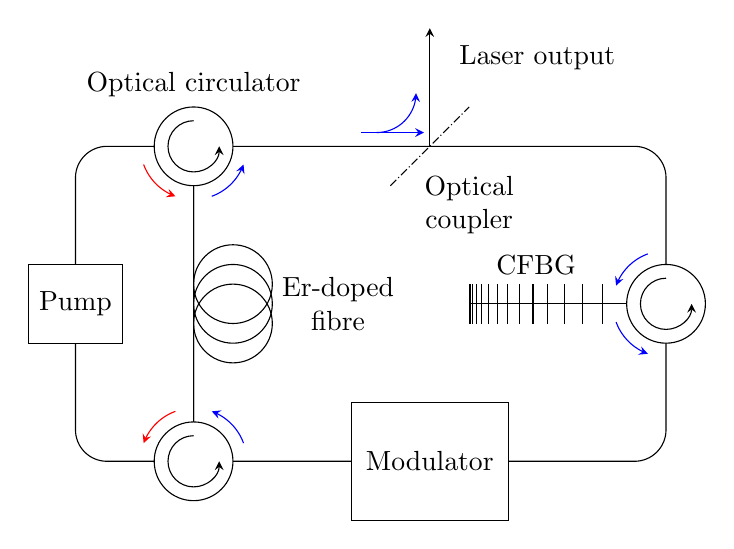
\begin{tikzpicture}
% Two laser loops
\draw [rounded corners=4mm] (0,0) rectangle ++(6,4);
\draw [rounded corners=4mm] (0,0) rectangle ++(-1.5,4);

% Gain
\draw (0.5,2.25) circle (0.5cm);
\draw (0.5,2) circle (0.5cm) node [anchor=west,xshift=0.5cm,align=center] {Er-doped \\ fibre};
\draw (0.5,1.75) circle (0.5cm);

% Modulator and pump
\filldraw[fill=white, draw=black] (2,-0.75) rectangle ++(2,1.5) node [midway] {Modulator};
\filldraw[fill=white, draw=black] (-2.1,1.5) rectangle ++(1.2,1) node [midway] {Pump};

% Coupler and output
\draw[-stealth] (3,4) -- (3,5.5) node [pos=0.75,anchor=west,xshift=0.25cm] {Laser output};
\draw[densely dashdotted] (2.5,3.5) -- (3.5,4.5) node [pos=1,anchor=north,yshift=-0.75cm,align=center] {Optical \\ coupler};

% Circulators
\filldraw[fill=white, draw=black] (6,2) circle (0.5cm);
\draw[->,>=stealth] (6,2.325) arc (90:360:0.325cm);

\filldraw[fill=white, draw=black] (0,0) circle (0.5cm);
\draw[->,>=stealth] (0,0.325) arc (90:360:0.325cm);

\filldraw[fill=white, draw=black] (0,4) circle (0.5cm) node [anchor=south,align=center,yshift=0.5cm] {Optical circulator};
\draw[->,>=stealth] (0,4.325) arc (90:360:0.325cm);

% Arrows
\draw [->,>=stealth,domain=20:70,blue] plot ({0.675*cos(\x)}, {0.675*sin(\x)});
\draw [->,>=stealth,domain=110:160,red] plot ({0.675*cos(\x)}, {0.675*sin(\x)});
\draw [->,>=stealth,domain=110:160,blue] plot ({6+0.675*cos(\x)}, {2+0.675*sin(\x)});
\draw [->,>=stealth,domain=200:250,blue] plot ({6+0.675*cos(\x)}, {2+0.675*sin(\x)});
\draw [->,>=stealth,domain=200:250,red] plot ({0.675*cos(\x)}, {4+0.675*sin(\x)});
\draw [->,>=stealth,domain=290:340,blue] plot ({0.675*cos(\x)}, {4+0.675*sin(\x)});

\draw [->,>=stealth,domain=270:360,blue] plot ({2.325+0.5*cos(\x)}, {4.675+0.5*sin(\x)});
\draw [->,>=stealth,blue] (2.125, 4.675-0.5) -- (2.325+0.6, 4.675-0.5);

% Grating
\draw (5.5,2) -- (3.5,2) node [pos=0.5,anchor=south,yshift=0.25cm,xshift=-0.15cm] {CFBG};
\foreach \i in {0,...,13}
	\draw (3.5 + \i*\i/100,1.75) -- (3.5 + \i*\i/100,2.25);

\end{tikzpicture}
	\caption{Typical cavity of a fibre based tuneable laser. The laser pulses travel clockwise around each loop.}
	\label{fig:cavity}
\end{figure}

\subsection{Discrete Models}
\label{sec:discrete}
Unfortunately, \eqref{eq:meml} is not completely representative of the underlying physics within our laser cavity. In the derivation of \eqref{eq:meml} it is assumed each process affects the pulse continuously within the cavity. As highlighted by Figure \ref{fig:cavity}, this is a rather poor assumption. Within the cavity each effect is localized to its corresponding component: almost all of the dispersion happens within the CFBG \cite{agrawal2002}, the pulse is only amplified within the Erbium-doped fibre, etc. Thus, a better model is one where \eqref{eq:meml} is broken down into the individual components giving the effect of each `block' of the cavity. Each of the blocks can then be functionally composed together to give an iterative map for the effect of one round trip of the cavity. This ultimately transforms the differential equation into an algebraic equation.

Such a method was first proposed in 1955 by Cutler \cite{cutler} while analyzing a microwave regenerative pulse generator. This method was adapted for mode-locked lasers in 1969 by Siegman and Kuizenga \cite{kuizenga1970a, siegman}. Kuizenga and Siegman also had success experimentally validating their model \cite{kuizenga1970b, kuizenga1970}. The effects of the nonlinearity would not be considered until Martinez, Fork, and Gordon \cite{martinez1984, martinez1985} tried modelling passively mode-locked lasers. This issue has recently been readdressed by Burgoyne \cite{burgoyne2014} in the literature for tuneable lasers. In each of these models the effect of each block is described by a transfer function.

Despite the development of these block style models, several short-comings exist. The clearest is that none of these models have contained every block---either the nonlinearity or the modulation have been omitted. In the framework of tuneable lasers, each component plays a crucial role and the tuneable laser will not function correctly without the inclusion of all of the components. Another key drawback is that the functional operations of some of the components used in their models are phenomenological. While these functions are chosen based on the observed output, they are not necessarily consistent with the underlying physics. Finally, none of these previous models have been able to exhibit wave breaking.


\section{Model Derivation}
\label{sec:model}
Using the idea presented Section \ref{sec:discrete} we derive our model from \eqref{eq:nlse}; however, in the case of the modulation we consider the exact functional form to be determined by the laser operator. To accomplish this, we neglect all terms but one of the right side of \eqref{eq:nlse} and solve the simplified differential equation. This is reasonable since the gain, loss, dispersion, modulation, and nonlinear effects are localized to one section of the laser cavity.

To proceed we must choose the form of the amplification term, $g(A)$. We assume the gain has the form
\begin{align}
	g(A) &= \frac{g_0}{1 + E / \Es},& E &= \int_{-\infty}^\infty |A|^2 \, \df T,
	\label{eq:energy}
\end{align}
where $g_0$ is a small signal gain, $E$ is the energy of the pulse, and $\Es$ is the energy at which the gain begins to saturate \cite{bohun, burgoyne2014, haus1975, hausbook, haus1992, haus2000, haus1991, kartner, peng, shtyrina, silfvast, usechak, yarutkina}. This leads to
\begin{align}
	G(A;E) &= \left( \frac{\Es}{E} W \left( \frac{E}{\Es} \textrm{e}^{E/\Es} \textrm{e}^{g_0 L_g} \right) \right)^{1/2} A
\end{align}
for the amplification of the pulse within the Er-doped fibre. Continuing this process for the loss, dispersion, and nonlinearity yields
\begin{align}
	L(A) &= (1 - R) \textrm{e}^{- \alpha L_T}A, \\
	D(A) &= \FTi{\textrm{e}^{i \omega^2 L_D\beta_2/2} \FT{A}}, \\
	F(A) &= A \textrm{e}^{i \gamma |A|^2 L_f},
\end{align}
where $R$ is the reflectivity of the output coupler\footnote{Depending on the layout of the laser cavity the loss may instead take the form $L(A) = R \textrm{e}^{- \alpha L_T}A$.}, $L_T$ is the total length of the laser circuit, $L_D$ is the length of the dispersive medium, $L_f$ is the length of fibre, and where $\mathcal{F}$ denotes the Fourier transform. Finally, we must assume a form for the modulation. The modulation is considered to be applied externally in which ever way the operator sees fit. For simplicity the representation is taken as the Gaussian
\begin{align}
	M(A) &= \textrm{e}^{-T^2 / 2 T_M^2} A,
\end{align}
where $T_M$ is the characteristic width of the modulation.

\subsection{Non-Dimensionalization}
The structure of each process of the laser can be better understood by re-scaling the time, energy, and amplitude; this suggests the convenient scalings:
\begin{align}
	T &= T_M \widetilde{T},& E &= \Es \widetilde{E},& A &= \left( \frac{\Es}{T_M} \right)^{1/2} \widetilde{A}.
\end{align}
Revisiting each process map shows each process has a characteristic non-dimensional parameter. The new mappings---after dropping the tildes---are
\begin{equation}
	\begin{aligned}
		G(A) &= \left(E^{-1} W \left( a E \textrm{e}^{E}\right) \right)^{1/2} A, & F(A) &= A \textrm{e}^{i b |A|^2} \\
		D(A) &= \FTi{\textrm{e}^{i s^2 \omega^2} \FT{A}}, & L(A) &= h A, \\
		M(A) &= \textrm{e}^{-T^2 / 2} A,
		\label{eq:effects}
	\end{aligned}
\end{equation}
with the four dimensionless parameters,
\begin{equation}
	\begin{aligned}
		a &= \textrm{e}^{g_0 L_g} \sim 8 \times 10^3,& \qquad h &= (1 - R) \textrm{e}^{-\alpha L} \sim 0.04, \\
		b &= \gamma L_f \frac{\Es}{T_M} \sim 1,& \qquad s &= \sqrt{\frac{\beta_2 L_D}{2 T_M^2}} \sim 0.2,
		\label{eq:ndparam}
	\end{aligned}
\end{equation}
which characterize the behaviour of the laser. Nominal values for \eqref{eq:ndparam} can be found in \cite{agrawal2002, agrawal2013, bohun, burgoyne2014, burgoyneemail, finot, li, litchinitser, peng, shtyrina, tamura1993, tamura1996, tomlinson, usechak, yamashita, yarutkina}. Notice that the modulation is only characterized by $T_M$, and each other process has its own associated independent non-dimensional parameter.

% Table of parameter values
% \begin{table*}[tbp]
% 	\centering
% 	\begin{tabular}{lcll}
% 		\hline\noalign{\smallskip}
% 		Parameter & Symbol & Value & Sources \\
% 		\hline\noalign{\smallskip}
% 		Absorption of Fibre & $\alpha$ & $10^{-4}$--$0.3\text{ m}^{-1}$  & \cite{burgoyneemail, shtyrina, tomlinson, usechak, yarutkina} \\
% 		Fibre Dispersion & $\beta_2^f$ & $-50$--$50 \text{ ps}^2/ \text{km}$ & \cite{agrawal2002, agrawal2013, burgoyne2014, litchinitser, peng, yarutkina} \\
% 		Fibre Nonlinearity & $\gamma$ & $0.001$--$0.01 \text{ W}^{-1} \text{m}^{-1}$ & \cite{agrawal2013, finot, usechak, yarutkina} \\
% 		Grating Dispersion & $\beta_2^g L_D$ & $10$--$2000 \text{ ps}^2$ & \cite{agrawal2002, agrawal2013, burgoyne2014, li} \\
% 		Length of Cavity & $L_T$ & $10$--$100 \text{ m}$ & \cite{burgoyneemail, peng, tamura1996} \\
% 		Length of Fibre & $L_f$ & $0.15$--$1 \text{ m}$ & \cite{burgoyneemail} \\
% 		Length of Gain Fibre & $L_g$ & $2$--$3 \text{ m}$ & \cite{burgoyne2014, peng, shtyrina, tamura1993, yarutkina} \\
% 		Modulation Time & $T_M$ & $15$--$150 \text{ ps}$ & \cite{bohun, burgoyneemail, burgoyne2014} \\
% 		Reflectivity of Optical Coupler & $R$ & $0.1$--$0.9$ & \cite{burgoyneemail, li, peng,  tamura1993, tamura1996, yamashita} \\
% 		Saturation Energy & $\Es$ & $10^3$--$10^4 \text{ pJ}$ & \cite{burgoyneemail, usechak, yarutkina} \\
% 		Small Signal Gain & $g_0$ & $1$--$10 \text{ m}^{-1}$ & \cite{burgoyneemail, yarutkina} \\
% 		\noalign{\smallskip}\hline
% 	\end{tabular}
% 	\caption{Range of variation of various parameters.}
% 	\label{tab:values}
% \end{table*}

\subsection{Combining the Effects}
\label{sec:effects}

\begin{figure}[tbp]
	\centering
	\includegraphics{Evo}
	\caption{Evolution of the envelope during one round trip of the cavity. The pulse decays due to the output coupler, is dispersed by the CFBG, is modulated by the modulator, and finally amplified by the gain fibre (the nonlinearity does not alter the envelope). Note that this is not to scale.}
	\label{fig:cavityevo}
\end{figure}

Now that we have the algebraic effect of each section of the cavity, we are ready to compose each map together to give the effect of one round trip of the cavity. We must now consider the order of the components. As we are most interested in the output of the laser cavity, we shall start with the loss. We then pass the pulse through the CFBG followed by the modulator. The pulse then travels through the Er-doped fibre to be amplified, and finally we consider the effect of the nonlinearity. The nonlinearity must immediately follow the gain since this is the section of the cavity where the pulse has the highest energy, and by \eqref{eq:effects} the effect of the nonlinearity is proportional to the energy. Note that is this model, the permutation of the components is indeed important as the operators do not, in general, commute---this is in contrast to the models described in Section \ref{sec:discrete}. Moreover, we prefer the loss to follow the gain and nonlinearity as we wish to mitigate the length over which the nonlinearity has an effect, and maximize the output power. Functionally we denote one round trip of the cavity by
\begin{align}
	\mathcal{L}(A) = F(G(M(D(L(A))))).
\end{align}
 The pulse after one complete circuit of the laser cavity is then returned back into cavity to restart the process. A steady solution to this model is one in which the envelope and chirp are unchanged after traversing every component in the cavity---we are uninterested in the phase. That is, such that $\mathcal{L}(A) = A \textrm{e}^{i \phi}$---for some $\phi \in \mathbb{R}$. In Figure \ref{fig:cavityevo} we can see an example of the evolution of the envelope of the pulse during one round trip of the cavity.

\section{Results}

\subsection{Linear Solution}

\subsection{Nonlinear Solution and Wave Breaking}

\section{Conclusion}


\clearpage
\newpage




\section{Linear Solution}
In the case $b = 0$ a solution can be found analytically. We expect the solution will have the form of a Gaussian. There are a few reasons for this; the solution to the models presented in \cite{cutler, siegman, kuizenga1970a, martinez1984, martinez1985} were Gaussian, the equilibrium shape will be highly correlated to the shape of the modulation function, and since a Gaussian is a fixed point of the Fourier transform \cite{gradshteyn}.

To compute $\mathcal{L}(A)$, consider the pulse
\begin{align}
	A = \sqrt{P} \exp \left( -(1 + iC) \frac{T^2}{2 \sigma^2} \right) \textrm{e}^{i \phi_0},
	\label{eq:A0}
\end{align}
where $P$ is the peak power, $C$ is the chirp, $\sigma^2$ is the variance, and $\phi_0$ is the initial phase. This form is chosen because it resembles the envelope and linear chirping found by experiment ***cite. Having neglected the effect of the nonlinearity $\mathcal{L}(A)$ can be found analytically from the process mappings \eqref{eq:effects}. By assuming the pulse in \eqref{eq:A0} is in equilibrium, we find that the variance must satisfy
\begin{align}
	\sigma^8 + 4 s^4 \sigma^6 - 20 s^4 \sigma^4 + 32 s^4 \sigma^2 - 16 s^4 = 0.
	\label{eq:var}
\end{align}
As this expression is a quartic in $\sigma^2$ it has an analytic solution, namely,
\begin{equation}
	\begin{split}
		\sigma^2 = \sqrt{2} s \left( s^6 + 3s^2 + \sqrt{4 + s^4} \left( 1 + s^4 \right) \right)^{1/2} & \\
		- s^4 - s^2 & \sqrt{4 + s^4}.
		\label{eq:equilvar}
	\end{split}
\end{equation}
Moreover, by asymptotically expanding \eqref{eq:var} we find the useful relations
\begin{align}
	\sigma^2 &\sim
	\begin{cases}
		2s(1 - s) + \bigO{s^3} & s \rightarrow 0 \\
		1 - \frac{1}{4}s^{-4} + \frac{3}{8}s^{-8} + \bigO{s^{-12}} & s \rightarrow \infty.
	\end{cases}
\end{align}
Additionally, from the variance we can determine the behaviour of the chirp to be
\begin{align}
	C &\sim
	\begin{cases}
		1 - s + \frac{1}{2}s^2 + \bigO{s^3} & s \rightarrow 0 \\
		\frac{1}{2}s^{-2} - \frac{3}{8}s^{-6} + \bigO{s^{-10}} & s \rightarrow \infty.
	\end{cases}
\end{align}
The equilibrium energy and peak power can be computed from \label{eq:energy} to give
\begin{align}
	E = \frac{h^2 \left( 1 - \sigma^2 \right)^{1/2}}{1 - h^2 \left( 1 - \sigma^2 \right)^{1/2}} \log \left( a h^2 \left( 1 - \sigma^2 \right)^{1/2} \right),
\end{align}
and
\begin{align}
	P = \frac{W(a E \textrm{e}^E)}{\sqrt{\pi} \sigma},
	\label{eq:equilpower}
\end{align}
respectively.

\section{Nonlinear Solution}
We now consider the nonlinear case---when $b > 0$. In this case it becomes impossible to obtain an analytic result. Recall from \eqref{eq:effects} that the nonlinearity is a highly nonlinear operator, and attempting to compute the Fourier transform analytically of a pulse that has undergone this transformation is futile. Instead we resort to a numerical solution.




With the inclusion of the nonlinearity we generally find a similar solution to the linear case. An example of this is shown in Figure \ref{fig:nlstable}.

Instead, the magnitude of the Fourier transform has a unique weakly bi-modal shape. This deviation suggests the nonlinearity implants higher frequency oscillations into the pulse---a key observation in the coming subsections. Finally, we shall examine the derivative of the phase---essentially the chirp.

 In the nonlinear case, we recover this linear response for moderate values of $T$. However, for $|T| > 1$ the chirp begins to saturate. This is consistent with the experimental results \cite{chen, rothenberg, tomlinson}.

\begin{figure}[tb]
	\centering
	\begin{subfigure}{\columnwidth}
		\centering
		\includegraphics{Conv}
		\caption{Example of a pulse stabilizing from a seemingly random initial pulse shape ($s = 0.1$, $b = 1.0$, $E_0 = 0.1$, $a = 8000$, $h = 0.04$).}
		\label{fig:convevo}
	\end{subfigure} \\
	\begin{subfigure}{\columnwidth}
		\centering
		\includegraphics{Break}
		\caption{Example of a pulse destabilizing from a hyperbolic secant initial pulse ($s = 0.1$, $b = 1.6$, $E_0 = 0.1$, $a = 8000$, $h = 0.04$).}
		\label{fig:breakevo}
	\end{subfigure}
	\caption{Two extremes of the evolution of a pulse.}
	\label{fig:evolution}
\end{figure}

The noise in the energy exhibited for moderate to large values of $b$, and small values of $s$ is a phenomenon called \emph{wave breaking} \cite{agrawal2013, anderson, finot, rothenberg, tomlinson}. Wave breaking is not limited to just optics; wave breaking occurs in areas such as plasmas, transmission lines, and fluid dynamics \cite{rothenberg}. Wave breaking occurs because the pulse begins to interfere with itself in a way called SPM \cite{agrawal2002, agrawal2013, becker}. SPM occurs because the index of refraction is intensity dependent \cite{agrawal2002, becker, rothenberg, silfvast}, which leads to additional chirp across the pulse \cite{agrawal2013, anderson, rothenberg, silfvast}. This in turn causes higher order frequencies to be injected into the pulse \cite{agrawal2013, anderson}, as we saw in Figure \ref{fig:nlstable}. These high frequencies compound with each trip around the cavity becoming parasitic very quickly---Figure \ref{fig:break} highlights this. Notice that the difference between Figure \ref{fig:nlstable} and Figure \ref{fig:break} is a difference in $b$ of $0.05$---just enough to cross the boundary---this difference could be attributed to adding a few centimetres more of fibre between the gain and output coupler. \\

The left figures show the pulse after 11 trips around the cavity; in the Fourier transform it is clear that the contributions from higher frequencies has increased. We obtain comparable results as in the experiments \cite{anderson, rothenberg}. Additionally, the chirp starts losing its linearity causing it to start becoming unstable; the nature of this instability is again in agreement with the experiments \cite{anderson, rothenberg}. The parasitic nature of the high frequency contributions is evident by examining the right figures. After five additional trips around the cavity, the envelope of the pulse is much more rippled, and the real and imaginary parts become incoherent. Moreover, the Fourier transform has no clear structure and has essentially become noise. The chirp has grown to be highly oscillatory and unstable. Once the pulse has reached a state such as this, the envelope, Fourier transform, and chirp never reach a steady equilibrium state.


\begin{figure}[htbp]
	\centering
	\includegraphics{ParamSpaceErr}
	\caption{}
	\label{fig:error}
\end{figure}

\begin{figure}[htbp]
	\centering
	\includegraphics{ParamSpaceEnergy}
	\caption{}
	\label{fig:}
\end{figure}

To obtain a better understanding of how the pulse either converges to equilibrium, or diverges to wave breaking, we shall examine the difference between the envelopes of consecutive iterations. More precisely, we compute the error by
\begin{align}
	\textrm{E} = \frac{\| |A_i| - |A_{i-1}| \|_2}{\| A_{i-1} \|_2},
	\label{eq:error}
\end{align}
where $\| \cdot \|_2$ denotes the $L^2(\mathbb{R})$ norm, which is computed numerically using the trapezoid rule ($N = 2^{18}$). Notice as well that in the numerator we use the modulus of the pulses, again this is because we are uninterested in the phase shift between iterations. A plot of the error can be found in Figure \ref{fig:error}, with $i = 100$. The standard method would be to iterate until a fixed tolerance is reached, however, there are some reasons that make a fixed number of iterations preferable---as long as a sufficient number is chosen. The main reason is that this allows us to observe a richer structure than simply whether or not the tolerance had been reached by some maximum number of iterations. Additionally, incorrectly choosing the critical tolerance could easily lead to erroneous categorizations at points.

Unsurprisingly, the error is largest in the region where the wave breaks. As mentioned in the previous subsection, the pulse does not reach a stable state in this region. As a consequence the envelope varies drastically, which leads to this large error.




The last item we wish to consider is the order in which the components are placed. In Section \ref{sec:effects} a brief description for the choice of the order was given. We start with the loss component since this coincides with the output; the fibre nonlinearity follows the gain since this is where it has the largest impact; and the loss follows the nonlinearity in an attempt to mitigate its effect. Therefore, the loss is first, and the gain followed by the nonlinearity are last---leaving dispersion and modulation in the middle. We chose to put the dispersion block ahead of the modulator. However, there was no real reason behind this---modulation before dispersion is equally as valid---and in this subsection we explore the effect of modulating the pulse before it passes through the CFBG. \\

The result of this switch is shown in Figure \ref{fig:switch}. As a whole, unsurprisingly, we find the same behaviour and structure, however, there are some intriguing differences. Again, the structure and periodic nature of the boundary is similar to before, however, this boundary has shifted rightwards to a larger $s$ value. Additionally, within the unstable region the density of the contour lines is much greater---suggesting it is in some sense more chaotic and random than with the components in their original permutation. The final main difference between the two orderings, is that in this case the energy contours are no longer monotonic functions of $s$. Instead we find a parabolic shape on the top contour, and two lobes on the second contour. \\






\section{Conclusion}
Within this paper we developed a new nonlinear model for tuneable lasers. In order to better represent the underlying physics within the laser cavity the nonlinear Schr\"{o}dinger equation was reduced to simpler differential equations for each component of the laser. This led to a functional map that defines the effect of each component on a particular input pulse. These processes were then composed together to give an iterative mapping of the whole laser cavity. In a future publication we shall show the results obtained by this iterative mapping as well as discuss the dynamics exhibited by this model---including wave-breaking---to predict the conditions under which the pulse is stable and sustainable.


\bibliography{Ref}

\end{document}
